% Author: Mabel Delgado

\documentclass[18pt]{beamer}

% To accept special characters from the keyboard
\usepackage[utf8]{inputenc}
% To altere the language of the document
\usepackage[spanish]{babel}
% To include figures
\usepackage{graphicx}
% To write mathematical formulation
\usepackage{amsmath}
% To include special fonts in mathematical formulation
\usepackage{amsfonts}
% To include special symbols in the mathematical formulation
\usepackage{amssymb}
% To include links in the references
\usepackage{url}
% To use colors
\usepackage{xcolor}
% To use hyperreferences
\usepackage{hyperref}
% To display code snippets
\usepackage{listings}

% Hyperlinks colors customization
\hypersetup{
	colorlinks = true,
  	urlcolor = blue,
  	citecolor = blue,
  	linkcolor = white  
}

% Define a new footnote object (without marker/associated number)
\newcommand\blfootnote[1]{%
  \begingroup
  \renewcommand\thefootnote{}\footnote{#1}%
  \addtocounter{footnote}{-1}%
  \endgroup
}

% Use python as code
\lstset{basicstyle=\ttfamily,
		language=python,
		showstringspaces=false}

% Remove figure word from figures
\setbeamertemplate{caption}{\raggedright\insertcaption\par}

% Remove navigation symbols
\setbeamertemplate{navigation symbols}{}

% Theme
\usetheme{Copenhagen}

% Information to be included in the title page
\title{Trabajando con Python en Ciencia e Ingeniería}
\author{Mabel Delgado (@mabeldelgadob)}
\institute{PyDay Granada 2018}
\date{15 de diciembre de 2018}

\begin{document}

% TITLE
\begin{frame}
	\titlepage
\end{frame}

% SOBRE MÍ
\begin{frame}
	\frametitle{Un poco sobre mí...}
	\begin{columns}
		\column{.6\textwidth}
		\begin{itemize}
			\setlength\itemsep{0.7em}		
			\item Ingeniera aeronáutica.
			\item Métodos y herramientas para ensayos en vuelo de aviones.
			\item Programación, software libre.
			\item PyLadies Madrid.
			\item AeroPython.
			\item Asociación Python España.
			\item Django Girls (Cáceres, Palma, Málaga).
			\item Python Software Foundation.
		\end{itemize}
			
		\column{.4\textwidth}
		\centering
			
\includegraphics[width=2.5cm]{images/aeropython.png}\\
			
\includegraphics[width=4cm]{images/pyladiesmadrid_alargado.png}\\
			
\includegraphics[width=2cm]{images/python_spain.png}
			
\includegraphics[width=2cm]{images/django_girls.jpg}\\
			
\includegraphics[width=4cm]{images/psf.png}
		\end{columns}
\end{frame}


% ECOSISTEMA PYTHON CIENTÍFICO
\begin{frame}

	\frametitle{Ecosistema Python para ciencia e ingeniería}
	
	\begin{figure}
		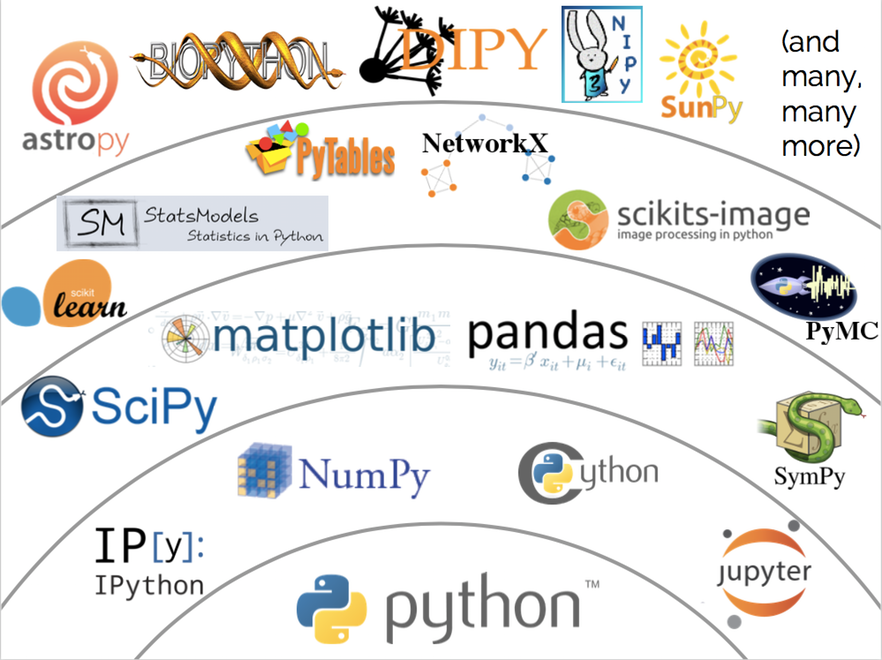
\includegraphics[width=8.8cm]{images/python_ecosystem.png}
	\end{figure}
	
	\blfootnote{\scriptsize https://www.datacamp.com/community/blog/python-scientific-computing-case}
	
\end{frame}


\begin{frame}

	\frametitle{Qué vamos a ver hoy...}
	
	\begin{itemize}
		\setlength\itemsep{0.7em}
		\item \textbf{NumPy} $\rightarrow$ arrays n-dimensionales.
		\item \textbf{SciPy} $\rightarrow$ algoritmos y funciones 
		 matemáticas.
		\item \textbf{Matplotlib} $\rightarrow$ representaciones 
		 gráficas 2D.
		%\item \textbf{SymPy} $\rightarrow$ matemática simbólica.
		\item \textbf{Jupyter (notebook, lab)} $\rightarrow$ entorno 
  		 interactivo de trabajo.
	\end{itemize}
                   
    \vspace{0.2cm}
                   
	Pero hay otros muchos paquetes que proporcionan desde funcionalidades
	generales (e.g. Pandas, SimPy, Numba, Bokeh...), a otras más
	específicas (Astropy, PyFiltering...).

\end{frame}


% NUMPY - INTRODUCCION
\begin{frame}

	\frametitle{NumPy - Introducción}

	\href{http://www.numpy.org/}{NumPy}
	es un paquete fundamental para la programación científica con Python,
	que proporciona un \textbf{objeto array n-dimensional}, para almacenar
	datos de forma eficiente, así como \textbf{funciones para trabajar con estos
	arrays}. 
	
	También incluye un módulo de álgebra lineal (\textbf{linalg}) para calcular; 
	determinante, inversa, autovalores y autovectores, etc.
	
	\vspace{0.4cm}
	
	\begin{figure}
		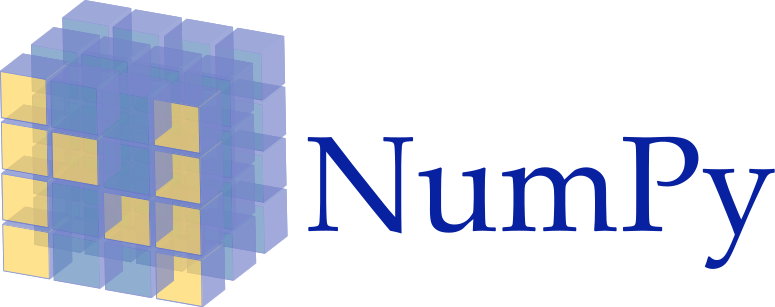
\includegraphics[width=4.2cm]{images/numpy.png}
	\end{figure}

\end{frame}


% NUMPY
\begin{frame}
	
	\frametitle{NumPy - Qué es un array}
	
	\centering
	\begin{figure}
		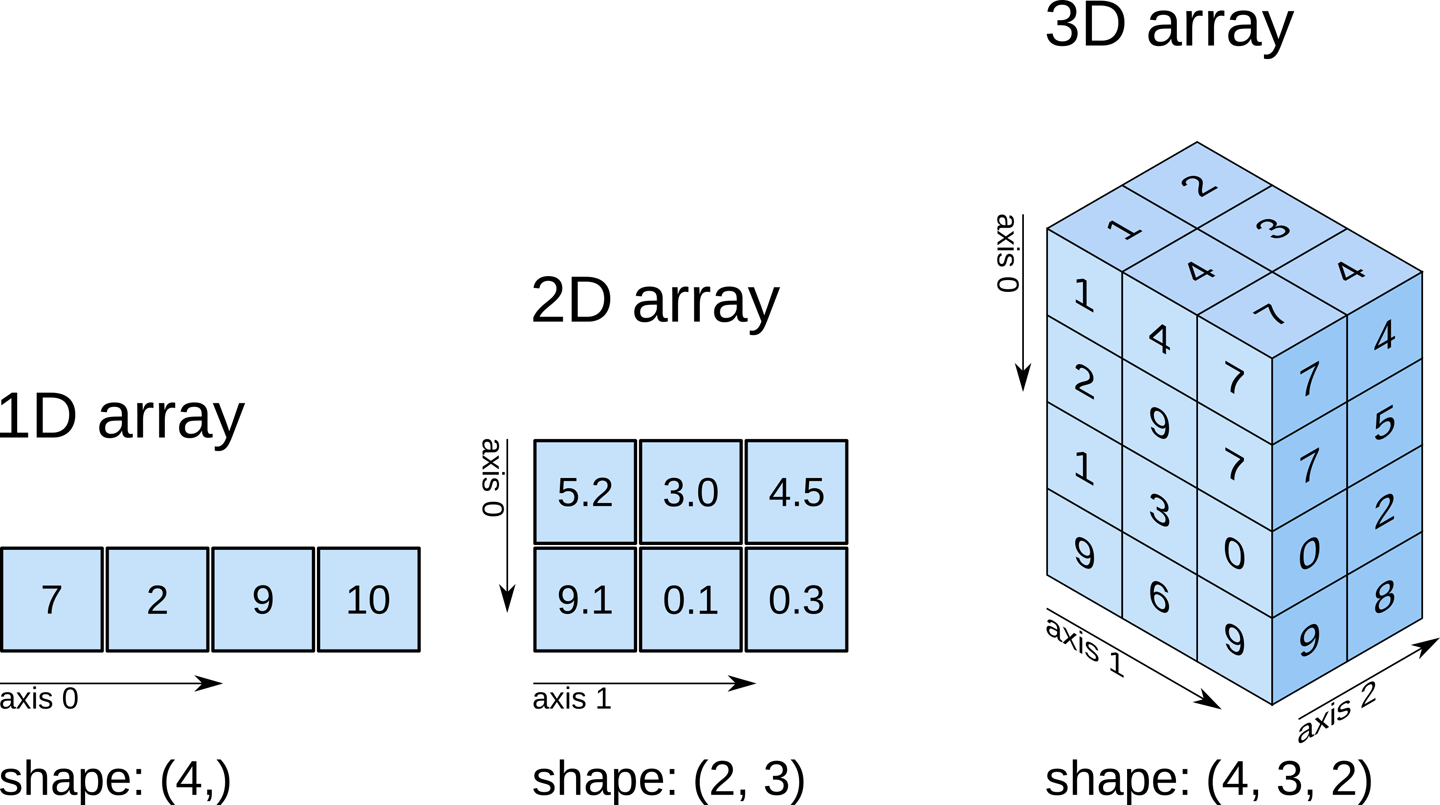
\includegraphics[width=9cm]{images/numpy_array_t.png}
	\end{figure}
	
	\blfootnote{\scriptsize https://www.oreilly.com/library/view/elegant-scipy/9781491922927/ch01.html}
		
\end{frame}


% NUMPY - CREACIÓN DE ARRAYS
\begin{frame}[fragile]
	
	\frametitle{NumPy - Creación de arrays (I)}
    
	\begin{itemize}
		\setlength\itemsep{0.3em}	
		\item Básica $\Rightarrow $ array, asarray
		\item Valores $\Rightarrow $ ones, zeros, full, empty
		\item Valores y forma $\Rightarrow $ ones\textunderscore like,
		 zeros\textunderscore like, full\textunderscore like, 
		 empty\textunderscore like
		\item Disposiciones especiales $\Rightarrow $ identity, eye, diag
		\item Secuencias $\Rightarrow $	arange, linspace, logspace
		\item Aleatorios $\Rightarrow $	numpy.random.randn,
		 numpy.random.randint...
		\item Desde fichero $\Rightarrow $ loadtxt (cuando no faltan 
		 valores), genfromtxt (cuando sí faltan valores)
				
	\end{itemize}

\end{frame}

% NUMPY - CREACIÓN DE ARRAYS
\begin{frame}[fragile]
	
	\frametitle{NumPy - Creación de arrays (II)}
		
	\begin{exampleblock}
	
		\small
	    \begin{lstlisting}
>>> import numpy as np
>>> np.array([1, 2+3j, 'hi', 7.5])
array(['1', '(2+3j)', 'hi', '7.5'], dtype='<U64')
>>> np.array([1, 2+3j, 7.5])
array([1. +0.j, 2. +3.j, 7.5+0.j])
    	\end{lstlisting}
    	
    \end{exampleblock}
      
   	\vspace{0.5cm}
    	
	\begin{alertblock}{¡¡Todos los elementos de un array son del mismo 
	tipo!!}
		Si se mezclan tipos en su creación, se usa el más
		 restrictivo. Esto recibe el nombre de upcasting.
	\end{alertblock}


\end{frame}


% NUMPY - OPERACIONES CON ARRAYS
\begin{frame}[fragile]

	\frametitle{NumPy - Operaciones con arrays}
	
	\begin{exampleblock}
		        
    	\small
    	\begin{lstlisting}
>>> import numpy as np
>>> a = np.array([[1, 2], 
                  [3, 4]])
>>> b = np.array([[4, 3], 
                  [2, 1]])
>>> a * b      # Multiplicacion elemen-wise
array([[4, 6],
       [6, 4]])
>>> a @ b      # Multiplicacion matricial
array([[ 8,  5],
       [20, 13]])
		\end{lstlisting}
		
	\end{exampleblock}

	\begin{alertblock}{Las operaciones; +, -, *, /, ... entre arrays 
	son elemento a elemento}
	
		La multiplicación matricial puede hacerse con 
		$np.dot(a, b)$ o con @
		
	\end{alertblock}	
	
\end{frame}


% NUMPY - SLICING
\begin{frame}[fragile]
	
	\frametitle{NumPy - Slicing (I)}
	
	\begin{itemize}
		\item El slicing permite extraer secciones de un array. 
	\end{itemize}
	
	\begin{block}
	
		\centering
		array[indice\_inicial:indice\_final:paso])
		
	\end{block}
				
	\begin{exampleblock}
		
    	\small
    	\begin{lstlisting}
>>> import numpy as np
>>> a = np.array([[1, 2, 3, 4], 
                  [5, 6, 7, 8], 
                  [9, 10, 11, 12]])
>>> a[0:3:2, ::3]
array([[1,    4],
       [   9,   12]])
		\end{lstlisting}
	\end{exampleblock}			
	
\end{frame}


% NUMPY - SLICING
\begin{frame}[fragile]
	
	\frametitle{NumPy - Slicing (II)}
			
	\begin{exampleblock}
		
    	\small
    	\begin{lstlisting}    
>>> b = a[0:3:2, ::3]
array([[1,    4],
       [   9,   12]])
>>> b[0, 0] = 9999
>>> b
array([[9999,    4],
       [   9,   12]])
>>> a
array([[9999,    2,    3,    4],
       [   5,    6,    7,    8],
       [   9,   10,   11,   12]])

		\end{lstlisting}
		
	\end{exampleblock}			


	\begin{alertblock}{¡¡Slicing devuelven una VIEW del array y NO una copia!!}		
		Si se modifican elementos de esa VIEW, se modifican también en el array
		 inicial. Para que esto no suceda, hay que usar .copy()
	\end{alertblock}	
		
\end{frame}


% NUMPY - RESHAPE
\begin{frame}[fragile]
	
	\frametitle{NumPy - Reshape (I)}

	\begin{itemize}
		\item La función reshape permite ver el array con una nueva forma. 
	\end{itemize}
	
	\begin{exampleblock}
			
    	\small
    	\begin{lstlisting}
>>> import numpy as np
>>> c = np.arange(6)
>>> c
array([0, 1, 2, 3, 4, 5])
>>> np.reshape(c, (2, 3))
array([[0, 1, 2],
       [3, 4, 5]])
		\end{lstlisting}
				
	\end{exampleblock}

	\begin{alertblock}{¡¡El reshape devuelve una VIEW del array inicial y NO una copia!!}		
		Si se modifican elementos del reshape, se modifican en el array inicial.
		Para que esto no suceda, hay que usar .copy()
	\end{alertblock}		

\end{frame}


\begin{frame}[fragile]
	
	\frametitle{NumPy - Reshape (II)}
	
	\begin{itemize}
		\item Utilización de reshape dejando 'libre' una dimensión		
	\end{itemize}
	
	\begin{exampleblock}
		
    	\small
    	\begin{lstlisting}
>>> np.reshape(c, (-1, 3))  # -1 dim libre 
array([[0, 1, 2],
       [3, 4, 5]])
>>> np.reshape(c, (-1, 2))
array([[0, 1],
       [2, 3],
       [4, 5]])
		\end{lstlisting}

	\end{exampleblock}

\end{frame}


% NUMPY - BROADCASTING
\begin{frame}
	
	\frametitle{NumPy - Broadcasting}

	\centering
	\begin{figure}
		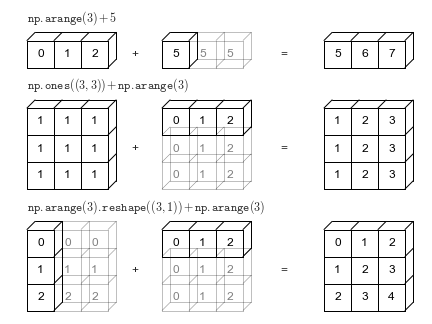
\includegraphics[width=8.5cm]{images/numpy-broadcasting.png}
	\end{figure}
	
	\blfootnote{\scriptsize https://jakevdp.github.io/PythonDataScienceHandbook/02.05-computation-on-arrays-broadcasting.html}
\end{frame}
	

% SCIPY - INTRODUCCIÓN
\begin{frame}

	\frametitle{SciPy - Introducción}

	\href{https://www.scipy.org/scipylib/index.html}{SciPy}
	es un paquete de Python que proporciona \textbf{funciones y 
	algoritmos matemáticos} destinadas al cálculo científico e 
	ingenieril. 
	Está construido sobre el paquete NumPy, y se estructura en diferentes 
	submódulos; \textbf{constants, linalg, optimize, etc.}
	
	\vspace{0.4cm}
	
	\begin{figure}
		
\includegraphics[width=4.0cm]{images/scipy.png}
	\end{figure}
	
\end{frame}


% SCIPY - ALGUNAS FUNCIONES DISPONIBLES
\begin{frame}
	
	\frametitle{SciPy - Submódulos disponibles en SciPy}

	\begin{itemize}
		\setlength\itemsep{0.3em}
		\item Funciones especiales (scipy.special)
		\item Integración (scipy.integrate)
		\item Optimización (scipy.optimize)
		\item Interpolación (scipy.interpolate)
		\item Transformadas de Fourier (scipy.fftpack)
		\item Procesamiento de señal (scipy.signal)
		\item Álgebra lineal (scipy.linalg)
		\item Matrices sparse (scipy.sparse)
		\item Estadística (scipy.stats)
		\item ...
	\end{itemize}
	
\end{frame}



% SCIPY - INTEGRACIÓN
\begin{frame}[fragile]
	
	\frametitle{SciPy - Integración}

	\begin{figure}
		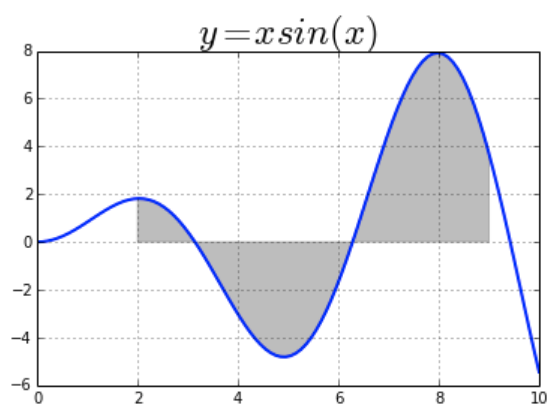
\includegraphics[width=3.9cm]{images/scipy_integrate.png}
	\end{figure}
	
	\begin{exampleblock}
	
    	\scriptsize
    	\begin{lstlisting}
>>> from scipy import integrate
>>> def fun(x): return x*np.sin(x)
>>> integrate.quad(fun, 2, 9)
(6.870699742283883,2.864870105641461e-13)
>>> x = np.linspace(2, 9,100)
>>> integrate.trapz(fun(x), x)
6.870667562274471
>>> integrate.simps(fun(x), x)
6.870699624669227
		\end{lstlisting}

	\end{exampleblock}
	
	\blfootnote{\scriptsize https://github.com/AeroPython/Curso\_AeroPython}

\end{frame}


% SCIPY - INTERPOLACIÓN
\begin{frame}[fragile]
	
	\frametitle{SciPy - Interpolación}

	\begin{figure}
		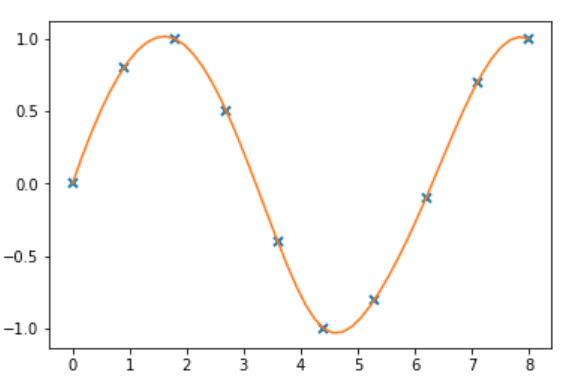
\includegraphics[width=4.8cm]{images/SciPy_interpolate.png}
	\end{figure}
	
	\begin{exampleblock}
	
    	\scriptsize
    	\begin{lstlisting}
>>> from scipy import interpolate
>>> x_i = [0., 0.9, 1.8, 2.7, 3.6, 4.4, 5.3, 6.2, 7.1, 8.]
>>> y_i = [0., 0.8, 1., 0.5, -0.4, -1., -0.8, -0.1, 0.7, 1.]
>>> f_interp = interpolate.interp1d(x_i, y_i, kind='cubic')
>>> x = np.linpace(0, 8)
>>> y = f_interp(x)
		\end{lstlisting}

	\end{exampleblock}
	
	\blfootnote{\scriptsize https://github.com/AeroPython/Curso\_AeroPython}
	
\end{frame}


% MATPLOTLIB - INTRODUCCIÓN
\begin{frame}

	\frametitle{matplotlib - Introducción}

	\href{https://matplotlib.org/}{matplotlib}
	es un paquete de \textbf{representación gráfica 2D} con Python, que 
	permite realizar figuras en una gran variedad de formatos, 
	incluidos entornos interactivos (e.g. jupyter notebook). 
	
	Es muy interesante su documentación, donde hay una galería con un 
	gran número de ejemplos y el código que los genera.
	
	\vspace{0.4cm}
	
	\begin{figure}
		
\includegraphics[width=6.0cm]{images/matplotlib.png}
	\end{figure}

\end{frame}


% MATPLOTLIB - REPRESENTACIONES BÁSICAS
\begin{frame}
	
	\frametitle{matplotlib - Subplots}

	\begin{columns}

		\column{0.75\textwidth}
			
		\begin{figure}
			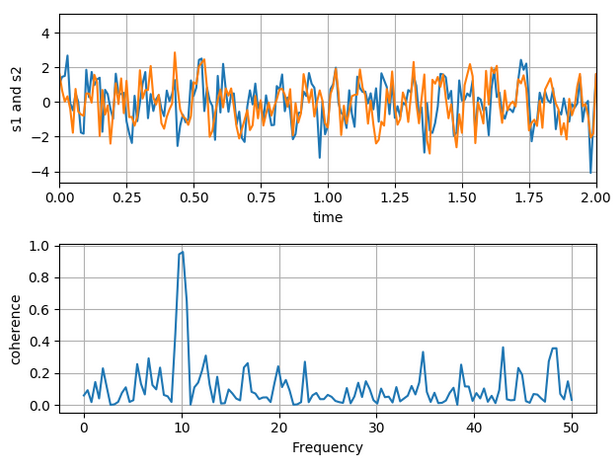
\includegraphics[width=7.5cm]{images/matplotlib_subplots.png}
		\end{figure}
	
		\column{0.25\textwidth}
			\begin{itemize}
				\item subplots
				\item xlabel, ylabel
				\item tight\_layout
			\end{itemize}
		
	\end{columns}
	
	\blfootnote{\scriptsize https://matplotlib.org/gallery/lines\_bars\_and\_markers/cohere.html\#sphx-glr-gallery-lines-bars-and-markers-cohere-py}
	
	% plots y subplots	
	
\end{frame}


% MATPLOTLIB - MAPAS DE CONTORNO
\begin{frame}
	
	\frametitle{matplotlib - Mapa de contorno}

	\begin{columns}
		\column{.65\textwidth}
			\centering
			\begin{figure}
				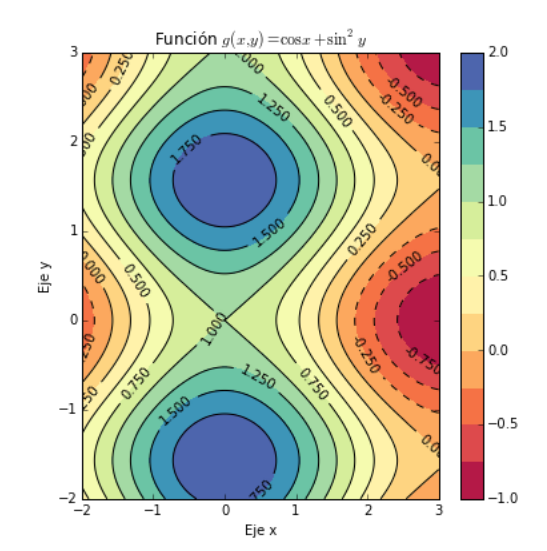
\includegraphics[width=6.8cm]{images/matplotlib_mapa_contorno.png}
			\end{figure}
			
		\column{.35\textwidth}
			\begin{itemize}
				\item contour
				\item contourf
				\item colorbar
				\item cmap
				\item clabel
			\end{itemize}
			
			\vspace{0.4cm}
			Además...
			\begin{itemize}
				\item np.linspace
				\item np.meshgrid
			\end{itemize}

	\end{columns}
	
	\blfootnote{\scriptsize https://github.com/AeroPython/Curso\_AeroPython}	
	
\end{frame}


% MATPLOTLIB - MATRICES E IMAGENES
\begin{frame}
	
	\frametitle{matplotlib - Matrices e Imágenes}
	
	\vspace{-1.5cm}	
	
	\begin{columns}

		\column{.5\textwidth}
			\centering
			\begin{figure}
				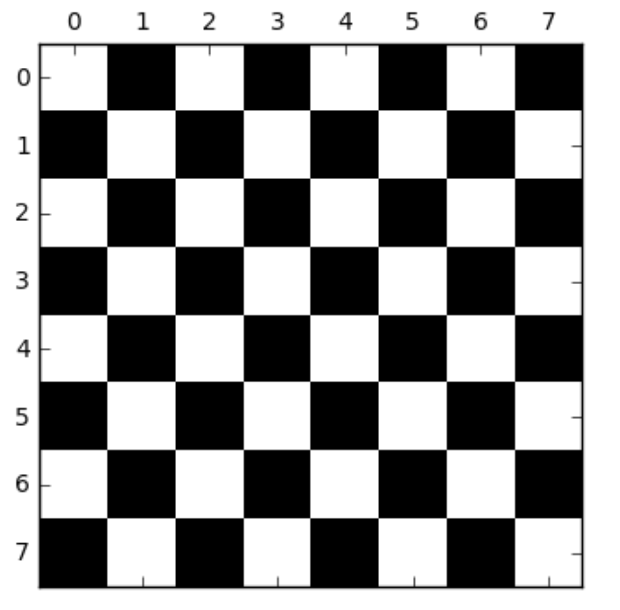
\includegraphics[height=3.8cm]{images/matplotlib_matshow.png}
			\end{figure}

			\vspace{-0.3cm}
			\begin{itemize}
				\item matshow
				\item cmap invertido (gray\_r)
			\end{itemize}
									
		\column{.5\textwidth}
			
			\vspace{0.6cm}
			\begin{figure}
				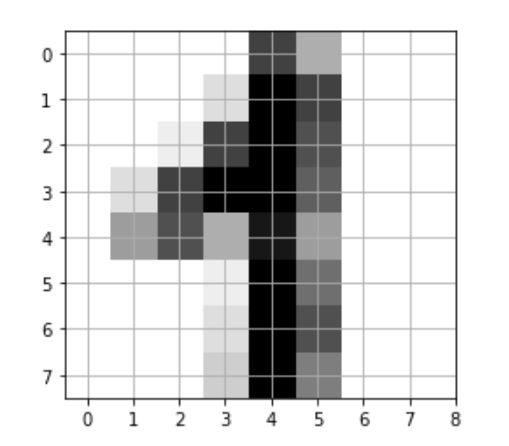
\includegraphics[height=4.0cm]{images/matplotlib_imshow.png}
			\end{figure}
			
			\vspace{-0.4cm}
			\begin{itemize}
				\item imshow
				\item grid
				\item xticks, yticks
			\end{itemize}

	\end{columns}

	\vspace{-2cm}	
	
	\blfootnote{\scriptsize https://github.com/AeroPython/Curso\_AeroPython}	
	
	\blfootnote{\scriptsize https://matplotlib.org/gallery/images\_contours\_and\_fields/
	interpolation\_methods.html}
	
\end{frame}


% MATPLOTLIB - CURIOSIDADES
\begin{frame}
	
	\frametitle{matplotlib - Curiosidades}

	\begin{columns}

		\column{.5\textwidth}
			\centering
			\begin{figure}
				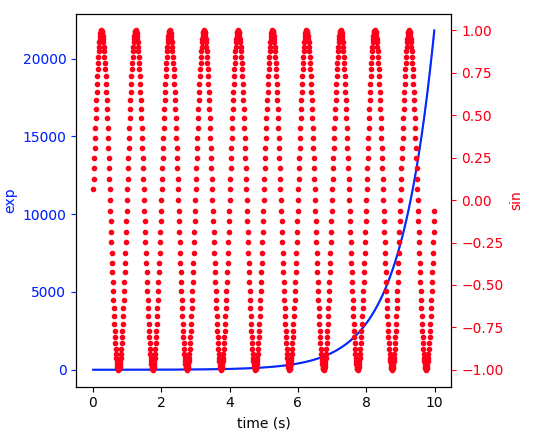
\includegraphics[height=4.2cm]{images/matplotlib_two_scales.png}
			\end{figure}

			\vspace{-0.5cm}
			\begin{itemize}
				\item twinx
				\item color yticks
				\item color ylabel
			\end{itemize}
									
		\column{.5\textwidth}
			
			\centering
			\begin{figure}
				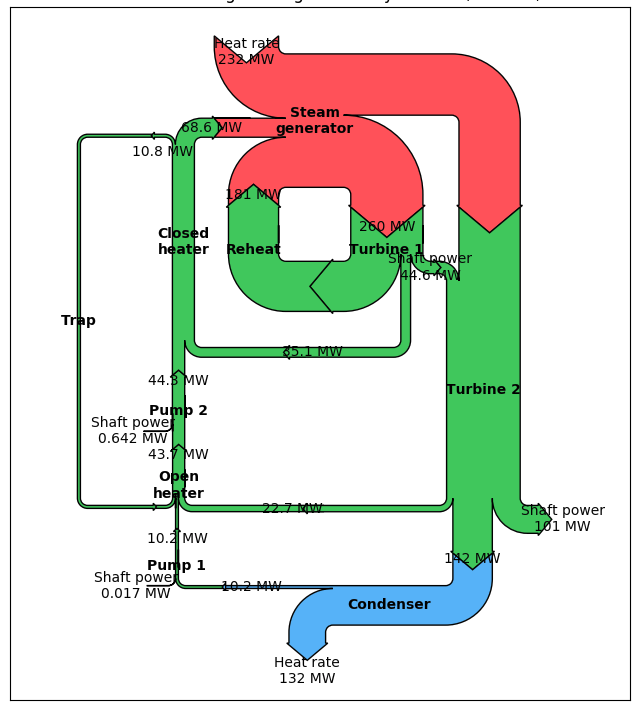
\includegraphics[height=5.8cm]{images/matplotlib_sankey_2.png}
			\end{figure}
			
			\vspace{-0.5cm}
			\begin{itemize}
				\item sankey
			\end{itemize}
	
	\end{columns}

	\blfootnote{\scriptsize https://matplotlib.org/examples/api/two\_scales.html}
	\blfootnote{\scriptsize https://matplotlib.org/examples/api/sankey\_demo\_rankine.html}	
	
\end{frame}


% JUPYTER NOTEBOOK/ JUPYTERLAB - INTRODUCCIÓN
\begin{frame}

	\frametitle{Jupyter notebook / JupyterLab - Introducción}

	\href{https://jupyter-notebook.readthedocs.io/en/stable/}{Jupyter 
	notebook} y  
	\href{https://jupyterlab.readthedocs.io/en/latest/}{JupyterLab} 
	son dos entornos interactivos que permiten crear y compartir documentos 
	que contienen código, texto, visualizaciones, etc.
	Ambos pertencen al proyecto jupyter, y aunque pueden ejecutar dentro 
	distintos kernels, se necesita haber instalado jupyter previamente con Python. 
	
	\vspace{0.4cm}
	
	\begin{figure}
		
\includegraphics[width=3.0cm]{images/jupyter.png}
	\end{figure}

\end{frame}


% JUPYTER NOTEBOOK / JUPYTERLAB - Prototipado
\begin{frame}
	
	\frametitle{Jupyter notebook / JupyterLab - Interfaz}

	% se puede customizar tocando el css
	% notebook vas a desaparecer.
	% se pueden abrir archivos de texto, csv, etc
	% Se pueden DDBB también??	
	\begin{figure}
		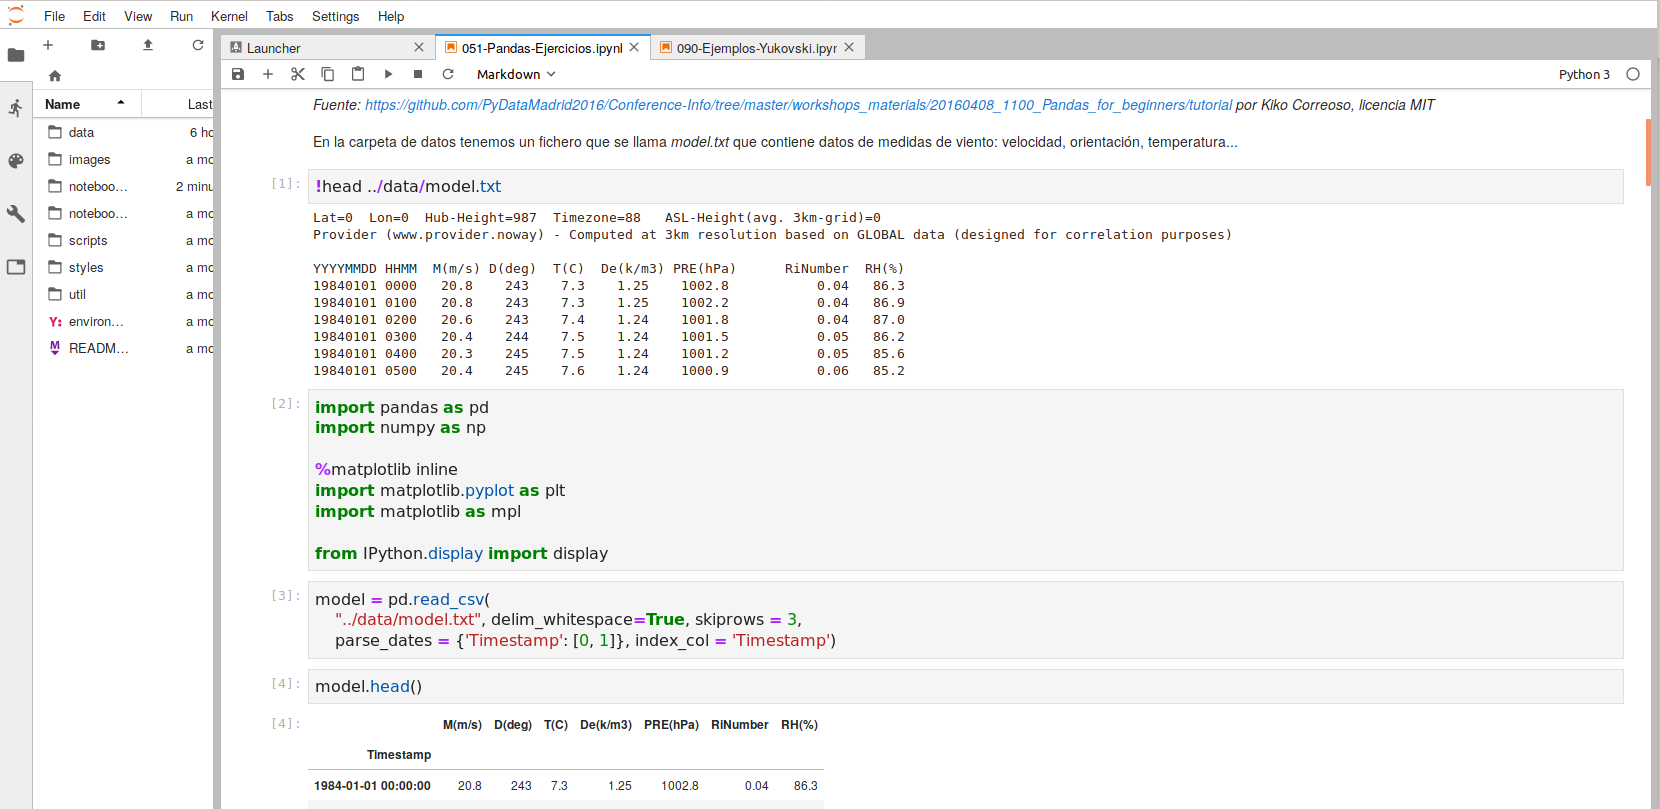
\includegraphics[scale=0.18]{images/prototipar.png}
	\end{figure}

	\blfootnote{\scriptsize https://github.com/AeroPython/Curso\_AeroPython}
	
\end{frame}


% JUPYTER NOTEBOOK / JUPYTERLAB - Usos
\begin{frame}
	
	\frametitle{Jupyter notebook / JupyterLab - Características}

	\begin{itemize}
		\setlength\itemsep{0.3em}
		\item Formado por \textbf{celdas} que ejecuta el kernel.
		\item \textbf{Diferentes lenguajes} para el kernel;
		 Python, R, Scala...
		\item Celdas de \textbf{código, texto (markdown), 
		imágenes, vídeos...}
		\item \textbf{Plots} se representan integrados en el notebook.
		\item Representaciones interactivas (\textbf{widgets}).
		\item \textbf{Interactuar con la terminal} del sistema operativo 
		($!<comando>$). e.g. !head  o !type, !ls o !dir, ...
		\item \textbf{'Magic commands'} que dan	funcionalidad 
		extra ($\%<comando>$). e.g. \%matplotlib notebook, \%timeit, ...
		\item Ejemplos de uso: aprendizaje, prototipado, representación 
		 de datos (plots y widgets), preparación lectura de ficheros ...
	\end{itemize}
	
\end{frame}



% PREGUNTAS
\begin{frame}

	\frametitle{¿Dudas? ¿Preguntas?}
	
	\begin{figure}
		% https://pixabay.com/en/airplane-takeoff-plane-2745898/
		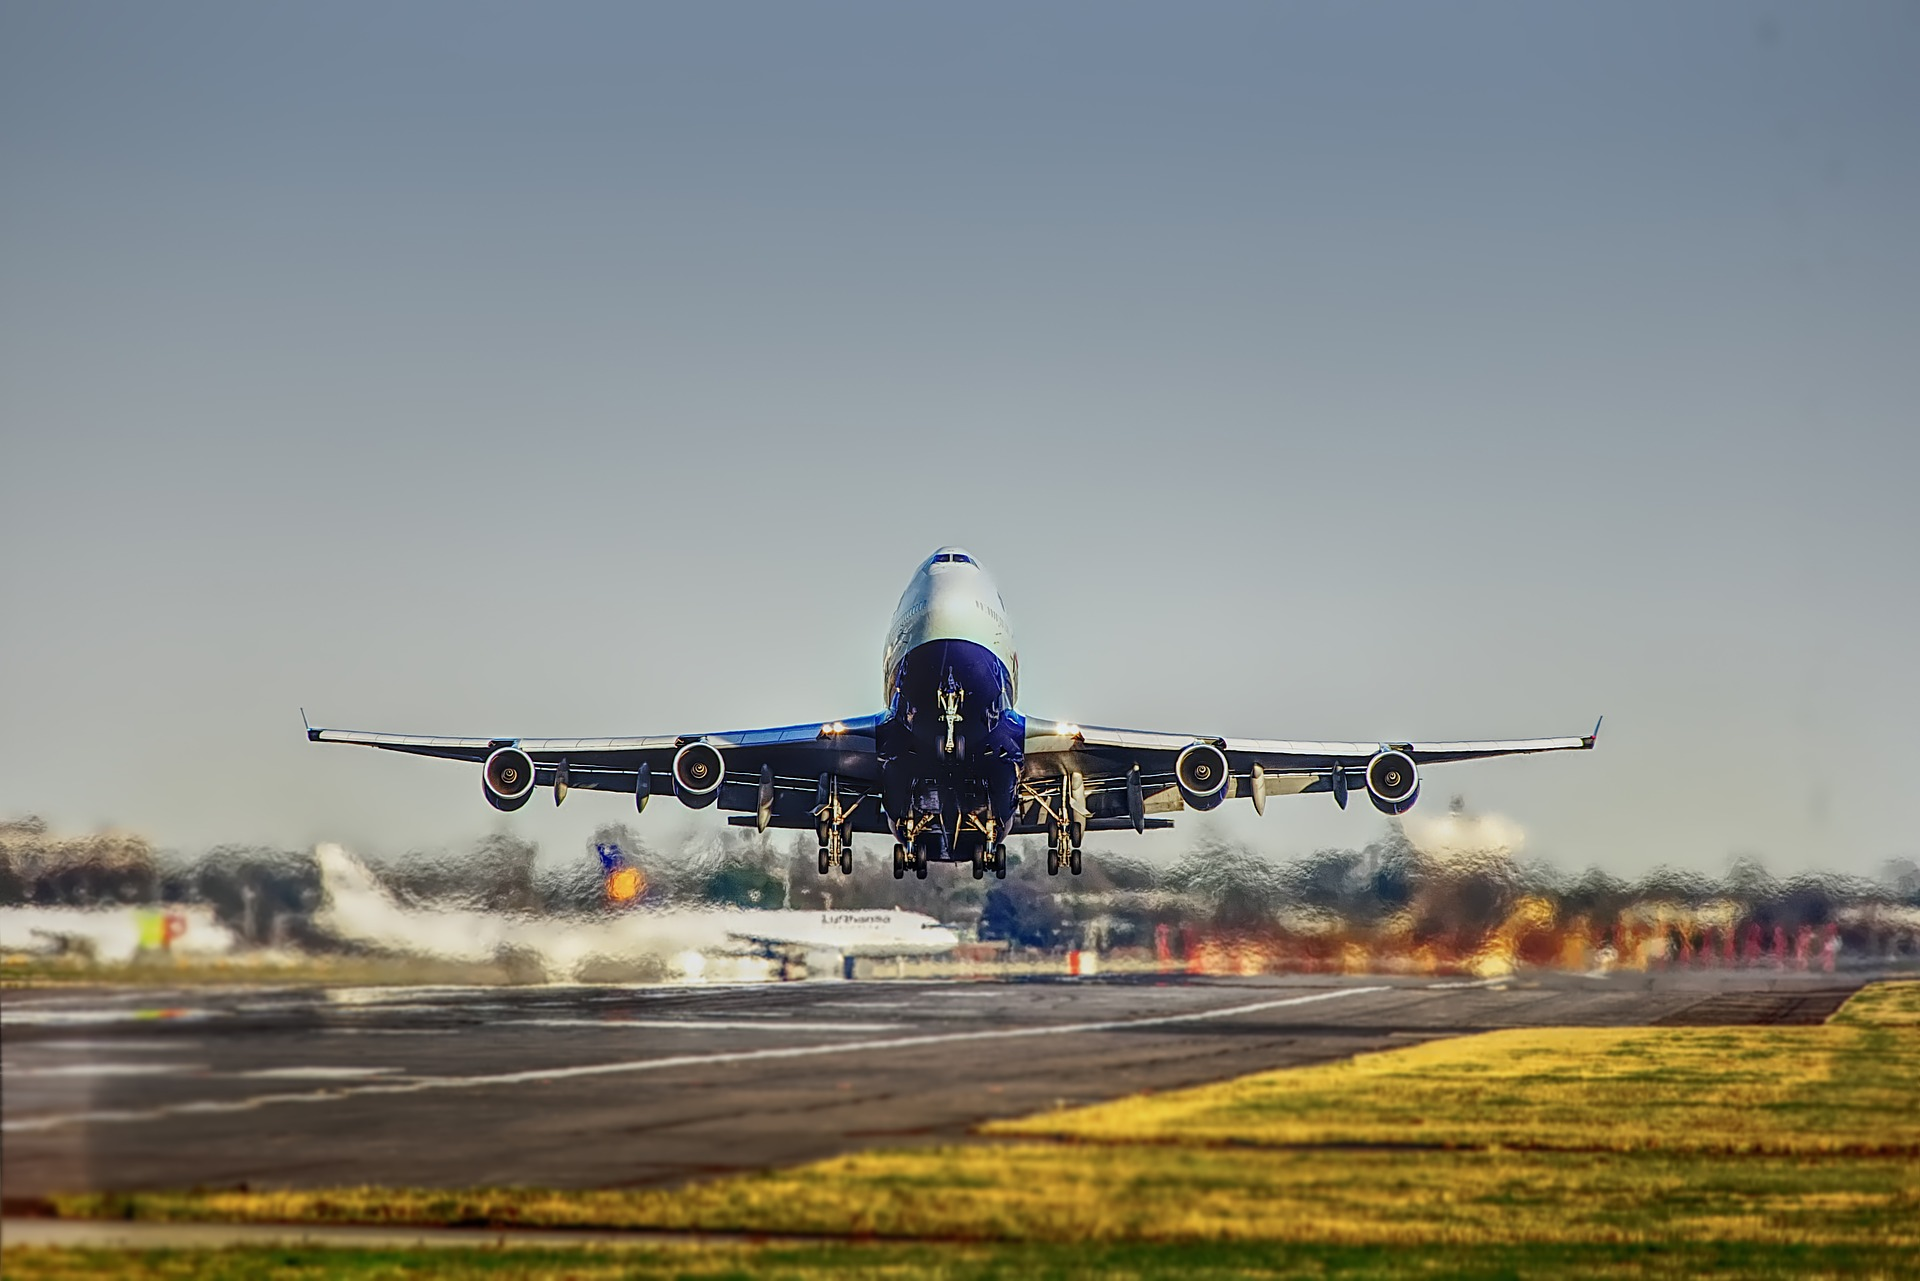
\includegraphics[width=8cm]{images/aircraft.jpg}
	\end{figure}

	\begin{center}
		\Large ¡Gracias por asistir!
	\end{center}
	
\end{frame}

	
\end{document}